\chapter{Software architecture}
The following sections present the software architecture of Modulo7.
\section{Server Side architecture}
\noindent Modulo7 is designed with the purpose of scalability. A block diagram of the components of the server side architecture is presented below :-
\begin{enumerate}
\item Source Converter : Converts music sources (e.g. music XML, midi etc) into modulo7's binary representation.
\item Music Theory Models : The model is a description of music theoretic criteria that can be applied on top of a song. Examples would be melodic contour, tonal histogram etc. 
\item Distributed Storage Mechanism : The modulo7 internal representation is a conversion to create a song representation with all the meta data of the song (Key, Scale,  etc) along with the sequences of note events stored as lists. This representation is then serialized and stored in and Hadoop Distributed File System. This allows for fault tolerance and a distributed deployment of the input data.
\item Lyrics Indexer : A distributed index of songs lyrics. This acts as a base on which standard techniques for similarity analysis might be applied. Alternatively it can provide a framework on which custom models (e.g. semantic intent of the song, correlation between music theory models and lyrics might also be applied).  
\item Lyrics similarity models : A set of similarity models that can be applied to an index. 
\item Query Engine : An SQL like interface to a client that allows you to gather and ascertain useful information (based on music theoretic criteria). 
\end{enumerate}

\begin{figure}[t]
\centering
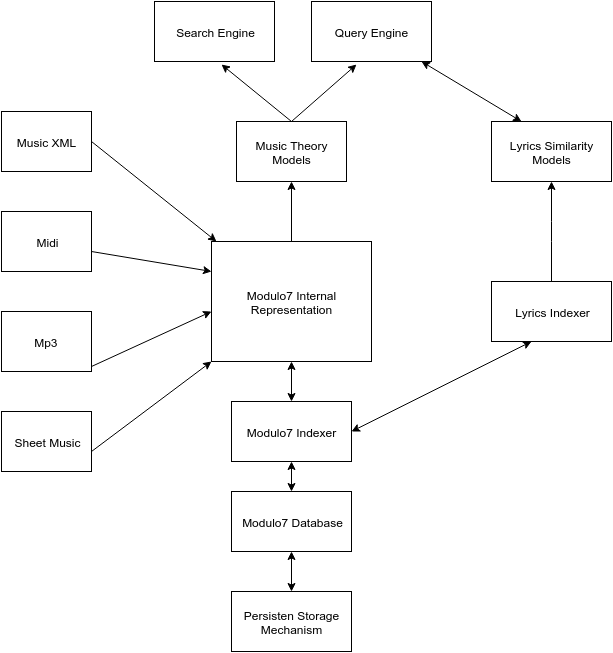
\includegraphics[width=\textwidth]{Modulo7Architecture.png}
\makeatletter
\let\@currsize\normalsize
\caption{Modulo7 architectural design}
\label{fig:figure}
\end{figure}
\section{Client architecture}
The server exposes a sql like interface as well as a consumable API. Some sample queries would be :-
\begin{enumerate}
\item select midi files from database where $melodic\_complexity > some threshold$
\item select * from database where $artist = led\_zepplin \ and \ harmonic\_movement > harmonic\_movement(stairway\_to\_heaven)$
\item select $ num\_voices \ from \ Database \ where \ songName = someSong.midi$ 
\end{enumerate}

An API will also be exposed to the client along a remote invocation procedure. The API would primarily target single sources for specifics. Some example API would be :-
\begin{enumerate}
\item int getNumVoices(String midiFilePath)
\item double melodicContourMovement(String pngSheetFilePath)
\item double compareAverageAttack(String musicXMLFile)
\end{enumerate}

This API can be consumed for specific song analysis. As design this API will not work on a bulk of files like its sql counterpart. 